\chapter{Phương pháp tiếp cận}

\section{Xây dựng tập dữ liệu}
\subsection{Xác đinh yêu cầu bài toán}
Bài toán đặt ra là nhận diện người trong khung hình có đang đeo các thiêt bị bảo hộ cá nhân (tiếng Anh: personal protective equipment) hay không. Các thiết bị bảo hộ cá nhân được chọn để nhận diện là: mũ bảo hộ, áo bảo hộ và khẩu trang.
\begin{figure}[ht!]
	\centerline{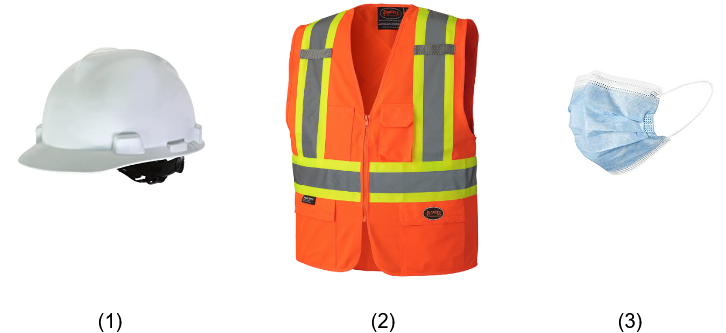
\includegraphics[scale=0.3]{images/ppe.png}}
  	\caption{(1) Mũ bảo hộ, (2) Áo bảo hộ, (3) Khẩu trang}
  	\label{fig:ppe}
\end{figure}

Mục tiêu đầu ra của hệ thống là có thể xác định được vị trí đầu người và thân người và phân loại việc sử dụng các thiêt bị bảo hộ cá nhận đối với các vật thể đã được phát hiện. Ứng với mỗi thiết bị, vật thể sẽ được phân loại thành hai trạng thái, một là \emph{Wearing} - \emph{Mặc}, hai là \emph{Not wearing} - \emph{Không mặc}.
\begin{itemize}
	\item Wearing a hardhat
	\item Not wearing a hardhat
	\item Wearing a safety vest
	\item Not wearing a safety vest
	\item Wearing a mask
	\item Not wearing a mask
\end{itemize}
Hình \ref{fig:expected_output} minh họa đầu vào đầu ra mong muốn của hệ thống.
\begin{figure}[ht!]
	\centerline{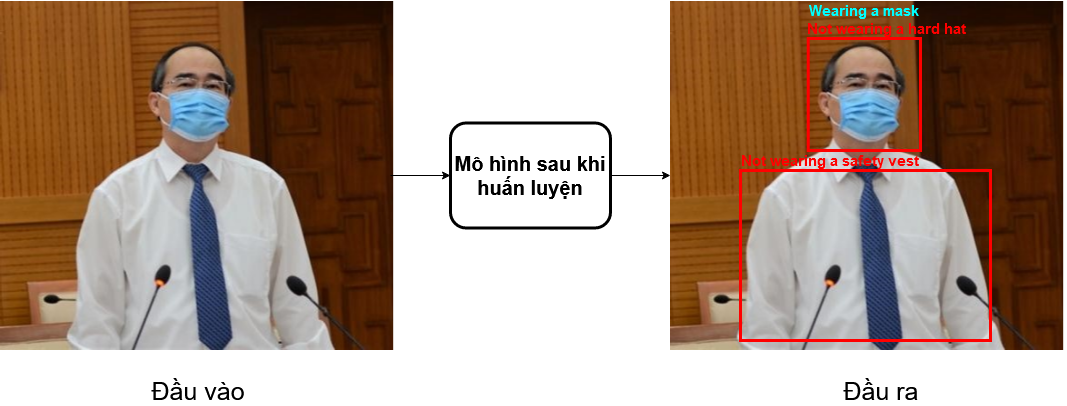
\includegraphics[scale=0.3]{images/expected_output.png}}
  	\caption{Kết quả nhận dạng mong muốn.}
  	\label{fig:expected_output}
\end{figure}

Do vậy tập dữ liệu sẽ được xậy dựng với các hình ảnh chứa con người và các nhãn được đánh đúng với mong muốn của đầu ra.
\subsection{Thu thập hình ảnh và dán nhãn}
Tập dữ liệu gồm $11586$ hình trong đó
\begin{itemize}
	\item $3541$ hình được lấy từ tập dữ liệu \emph{Hardhat and Safety Vest Image for Object Detection}
	\item $3174$ hình được lấy từ tập dữ liệu \emph{GDUT-HWD}
	\item $4871$ hình được lấy từ công cụ tìm kiếm hình ảnh \emph{Google image}
\end{itemize}

Các hình được dán nhãn bằng phần mềm \emph{LabelImg}. Mỗi hình sẽ có tương ứng một tệp tin văn bản với đuôi \emph{.txt}. Bên trong tệp tin này là các nhãn được đánh dấu bằng định dạng của YOLO với các thông tin gồm \emph{object class id} - đây là id tương ứng với thứ tự của một nhãn trong danh sách các nhãn, \emph{x} và \emph{y} là tọa độ tương đối của bounding box được đánh dấu với hình, \emph{w} và \emph{h} là chiều rộng và chiều cao tương đối của bounding box được đánh dấu với hình, hình \ref{fig:}.
\begin{figure}[ht!]
	\centerline{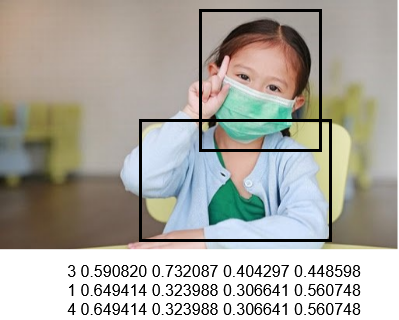
\includegraphics[scale=0.6]{images/yolo_annotation.png}}
  	\caption{Định dạng nhãn của YOLO.}
  	\label{fig:yolo_annotation}
\end{figure}

Tập dữ liệu này có tổng cộng $195771$ vật thể được dán nhãn với thống kê số vật thể của từng class được thể hiện trong hình \ref{fig:object_count}.
\begin{figure}[ht!]
	\centerline{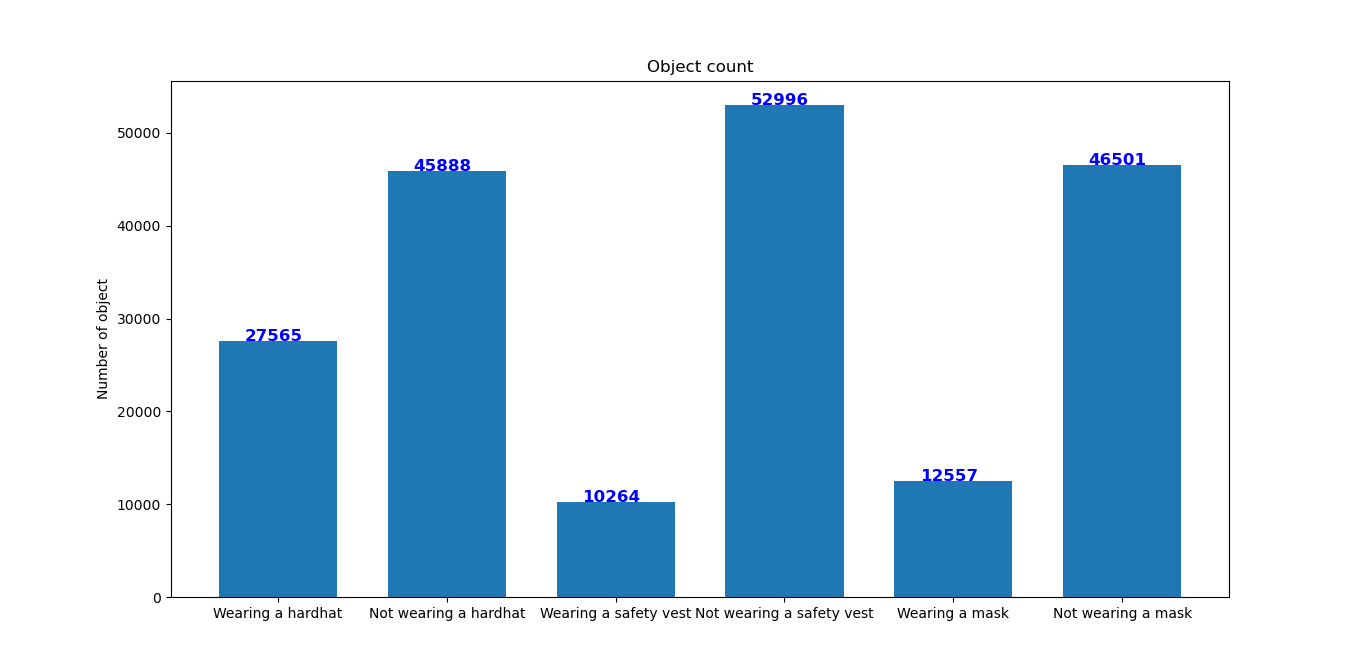
\includegraphics[scale=0.5]{images/object_count.png}}
  	\caption{Thống kê số lượng vật thể ứng với từng class. Wearing a hardhat: $27565$, Not wearing a hardhat: $45888$, Wearing a safety vest: $10264$, Not wearing a safety vest: $52996$, Wearing a mask:$12557$, Not wearing a mask: $46501$.}
  	\label{fig:object_count}
\end{figure}

Việc chênh lệch lớn về số lượng các bounding box giữa các class cụ thể là các class \emph{Not wearing} có số lượng lớn hơn rất nhiều so với các class \emph{Wearing} tương ứng sẽ giúp bộ nhận dạng nhạy hơn với các trường hợp vi phạm trang phục bảo vệ lao động. Tuy có sự chênh lệch lớn nhưng số lượng các bounding box của mỗi class là đủ lớn để mô hình có thể học được các đặc trưng cần thiết để có thể phân loại class tốt cho một bounding box.

\section{Huấn luyên mạng YOLOv3 sử dụng framework Darknet}
Darknet là một framework được xây dựng bởi Joseph Redmon cũng là cha đẻ của YOLO, framework này được viết bằng C/C++ và được dùng để huấn luyện mô hình YOLOv3 với tâp dữ liệu riêng cho từng vấn đề. Kiến trúc của Darknet đã được đề cập ở phần lý thuyết và sẽ không được nhắc lai ở chương này.

Mô hình YOLOv3 trong luận văn này được huấn luyện trên $Google Colab$, về bản chất môi trường trên $Google Colab$ là môi trường máy ảo chạy Linux với các thông số tại thời điểm thực hiện luận văn: 
\begin{itemize}
	\item Hệ điều hành: Ubuntu 18.04.3 LTS
	\item Chip xử lý: Intel 2-core Xeon 2.2GHz
	\item RAM: 13Gb
	\item HDD: 33Gb
	\item GPU: Tesla K80 with 12GB memory
\end{itemize}

Để có thể huấn luyện được mô hình YOLOv3 cho bộ dữ liệu riêng, ta cần thực hiện một số bước.
\begin{enumerate}
	\item Tải framework Darknet từ github repository của \href{https://github.com/AlexeyAB/darknet}{AlexeyAB}.
	
\noindent\fbox{
    \parbox{\textwidth}{
        https://github.com/AlexeyAB/darknet
    }
}

	Sau đó ta chọn Clone $\rightarrow$ Download ZIP và tiến hành tải thư mục về, sau khi tải xong ta tiến hành giải nén vào một thư mục mà ta tạo sẵn.
	\item Ta chép tệp tin \emph{yolov3.cfg} trong thư mục \emph{cfg} ra thư mục làm việc hiện tại và chỉnh sửa như sau. Đầu tiên ta sẽ sửa các giá trị \emph{batch} là số hình trong một mini-batch mà ta muốn dùng để huấn luyện, \emph{subdivision} là thông số để chia nhỏ một mini-batch để đảm bảo mô hình có thể chạy trên các tài nguyên GPU khác nhau, \emph{width} và \emph{height} là chiều rộng và chiều cao của ảnh đầu vào, các ảnh có kích thước khác nhau sẽ được resize lại kích thước này trước khi được đưa vào để huấn luyện. \emph{max{\_}batches} là tổng số batch mà mô hình sẽ chạy qua, đây còn được gọi là số \emph{iteration}. \emph{steps} sẽ có giá trị lần lượt băng $80\%$ và $90\%$ của \emph{max{\_}batches}.

\noindent\fbox{
    \parbox{\textwidth}{
        \texttt{\#} [net]\\
		\texttt{\#} Testing\\
		\texttt{\#} batch=1\\
		\texttt{\#} subdivisions=1\\
		\texttt{\#} Training\\
		batch=64\\
		subdivisions=64\\
		width=608\\
		height=608\\
		channels=3\\
		momentum=0.9\\
		decay=0.0005\\
		angle=0\\
		saturation = 1.5\\
		exposure = 1.5\\
		hue=.1\\
\\
		learning{\_}rate=0.001\\
		burn{\_}in=1000\\
		max{\_}batches = 22000\\
		policy=steps\\
		steps=17600,19800\\
		scales=.1,.1\\
    }
}

Sau đó tại các dòng $610, 696$ và $783$ ta sẽ thay số $classes$ bằng sáu, chính là số class của bài toán. Đồng thời ta sẽ sửa số $filters$ của lớp convolution ngay phía trên theo công thức $3 \times (5+C)$ với $C$ là số class, khi $C=6$ ta có $filters=33$.

\noindent\fbox{
    \parbox{\textwidth}{
		[convolutional]\\
		size=1\\
		stride=1\\
		pad=1\\
		filters=33\\
		activation=linear\\
\\
		\text{[yolo]}\\
		mask = $0,1,2$\\
		anchors = $10,13,16,30,33,23,30,61,62,45,59,119,116,90,156,198,373,326$\\
		classes=6\\
		num=9\\
		jitter=.3\\
		ignore{\_}thresh = .7\\
		truth{\_}thresh = $1$\\
		random=$1$\\
	}
}

	\item Sửa các thông số ở đầu của tệp \emph{Makefile} như sau.

\noindent\fbox{
    \parbox{\textwidth}{
		GPU=1\\
		CUDNN=0\\
		CUDNN{\_}HALF=0\\
		OPENCV=1\\
		AVX=0\\
		OPENMP=0\\
		LIBSO=0\\
		ZED{\_}CAMERA=0 \# ZED SDK 3.0 and above\\
		ZED{\_}CAMERA{\_}v2{\_}8=0 \# ZED SDK 2.X\\
	}
}

	\item Tạo tệp có tên $obj.names$ chứa tên các class.

\noindent\fbox{
    \parbox{\textwidth}{
		Wearing a hardhat\\
		Not wearing a hardhat\\
		Wearing a safety vest\\
		Not wearing a safety vest\\
		Wearing a mask\\
		Not wearing a mask\
	}
}

	\item Tạo hai tệp text, $train.txt$ và $val.txt$ chứa đường dẫn đến các hình ảnh. $train.txt$ sẽ được dùng để huấn luyện còn $val.txt$ sẽ được dùng để validate mô hình trong quá trình huấn luyện. Việc chia tập dữ liệu được thực hiện ngẫu nhiên. Có $900$ hình được dùng để validate và $10686$ hình được dùng để huấn luyện. Việc chia này được thực hiện bằng một chương trình Python.

\noindent\fbox{
    \parbox{\textwidth}{
		import os\\
		import glob\\
		import cv2\\
		import random\\
\\
		basenames = \text{[os.path.basename(x) for x in glob.glob(".$/$data$/$objects$/$*.jpg")]}\\
		basenamesNotEmpty = []\\

		for name in basenames:\\
		    if "empty" not in name:\\
		    basenamesNotEmpty.append(name)\\

		train = random.sample(basenames, len(basenames))\\
		valid = random.sample(basenamesNotEmpty, 900)\\

		with open(".$/$val.txt","w") as f:\\
    		for name in valid:\\
        		f.write("data$/$objects$/$"+name+"$\backslash$n")\\
        
		with open(".$/$train.txt","w") as f:\\
			for name in train:\\
	        	if name not in valid:\\
		        f.write("data$/$objects$/$"+name+"$\backslash$n")\\
	}
}

	\item Tạo tệp có tên $obj.data$ chứa tên các class.

\noindent\fbox{
    \parbox{\textwidth}{
		classes = 6\\
		train = train.txt\\
		valid = val.txt\\
		names = obj.names\\
		backup = backup/\\
	}
}
\end{enumerate}